\begin{center}
    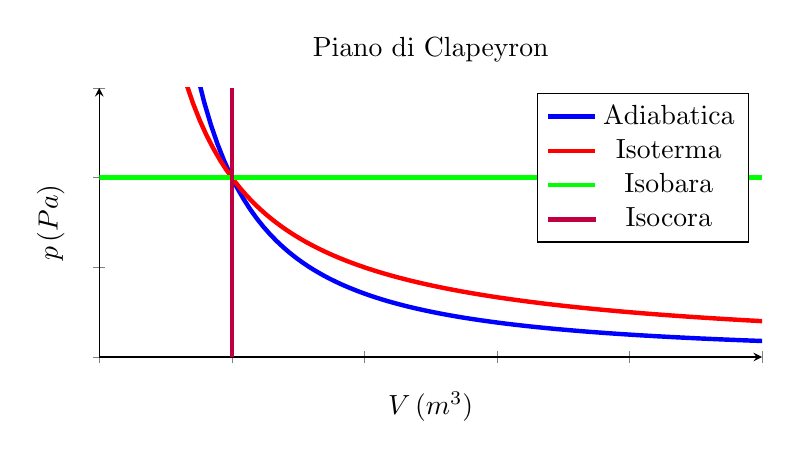
\begin{tikzpicture}
    
        \begin{axis}[
            title = Piano di Clapeyron,
            axis lines = left,
            xlabel = $V \, (m^3)$,
            ylabel = {$p \, (Pa) $},
            width= 10cm,
            height=5cm,
            ymax = 1.5,
            yticklabel=\empty,
            xticklabel = \empty
        ]
        
        \addplot [
            ultra thick,
            domain= .1:5, 
            samples=100, 
            color = blue,
        ]
        {pow(x, -(3/2))};
        \addlegendentry{Adiabatica}
        
        \addplot [
            ultra thick,
            domain= 0:5, 
            samples=100, 
            color = red,
        ]
        {1/x};
        \addlegendentry{Isoterma}
        
        
        \addplot [
            ultra thick,
            domain= 0:5, 
            samples=100, 
            color = green,
        ]
        {1};
        \addlegendentry{Isobara}
        
        \addplot[
            ultra thick, 
            samples=1, 
            smooth,
            domain=0:1,
            color = purple,
        ] coordinates {(1,0)(1,1.5)};
        \addlegendentry{Isocora}
        
        
        \end{axis}
    \end{tikzpicture}
\end{center}